\documentclass[11pt, oneside]{amsart}   	% use "amsart" instead of "article" for AMSLaTeX format
\usepackage{geometry}                		% See geometry.pdf to learn the layout options. There are lots.
\geometry{letterpaper}                   		% ... or a4paper or a5paper or ... 
%\geometry{landscape}                		% Activate for for rotated page geometry
%\usepackage[parfill]{parskip}    		% Activate to begin paragraphs with an empty line rather than an indent
\usepackage{graphicx}				% Use pdf, png, jpg, or eps� with pdflatex; use eps in DVI mode
								% TeX will automatically convert eps --> pdf in pdflatex		
\usepackage{amssymb}
\usepackage{listings}

\title{CS 325: Project 1}
\author{Group 29: Jacob Mastel, Yash Naik, Cera Olson}
\date{}							% Activate to display a given date or no date

\begin{document}
\maketitle
\section{Algorithm 1: Enumeration}
\subsection{Theoretical Run-Time Analysis}

Enumeration has a running time of $O(n^{3})$. Because of the 3 loops, each run n times gives the algorithm a running time of ${n*n*n}$.

\subsubsection{Pseudocode}
\begin{verbatim}
for i = 1 to n
	for j = i to n
		for k = i to j
			sum += $a_k$
		if  sum > ans then ans = sum
return ans
\end{verbatim}
\break
\break	
\subsection{Experimental Analysis}
\break
\break
\break
\begin{figure}
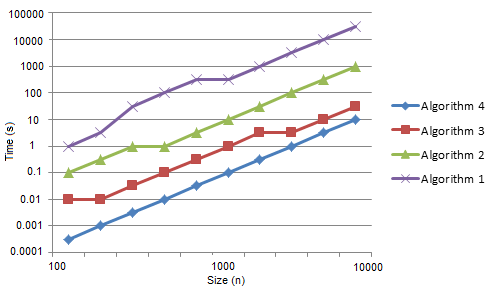
\includegraphics{AvgRunTime.png} 
\caption{Average Run Time for All 4 Algorithms}
\end{figure}
\break
\begin{figure}
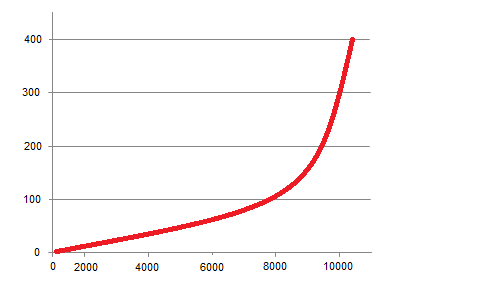
\includegraphics{Alg1Log.png}
\caption{Algorithm 1 Run Time}
\end{figure}

\begin{center}
\begin{tabular}{ |c|c| } 
 \hline
 n & Time \\ 
100	& 0.029255198\\
200	& 0.178765495\\
300	& 0.541698859\\
400	& 1.337829466\\
500	& 2.473190885\\
600	& 4.287970855\\
700	& 7.054050103\\
800	& 10.06102867\\
900	& 15.23538047\\
1000	 & 20.64124558\\
1100	 & 26.77310262\\
1200	 & 31.31654893\\
1300	 & 39.63601268\\
1400	 & 49.22060823\\
1500	 & 60.55456953\\
1600	 & 73.94340321\\
1700	 & 84.80297324\\
1800	 & 99.51908661\\
1900	 & 117.1002546\\
2000	 & 136.9574863\\
 \hline
\end{tabular}
\end{center}

\subsection{Extrapolation and Interpretation}

\subsubsection{For each algorithm use the experimental data to estimate a function that models the relationship between running times and input sizes (n). Discuss any discrepancies between the experimental and theoretical running times.}



\subsubsection{For each algorithm, what is the size of the biggest instance that you can solve with your algorithm in one hour?}

\section{Algorithm 2: Better Enumeration}
\subsection{Theoretical Run-Time Analysis}

\subsubsection{Pseudocode}
\begin{verbatim}
for i = 1 to n
	for j = i to n
		for k = i to j
			sum += $a_k$
		if  sum > ans then ans = sum
return ans
\end{verbatim}

\subsection{Experimental Analysis}
\begin{figure}
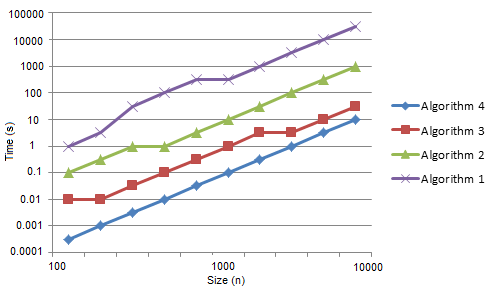
\includegraphics{AvgRunTime.png} 
\caption{Average Run Time for All 4 Algorithms}
\end{figure}
\break
\begin{figure}
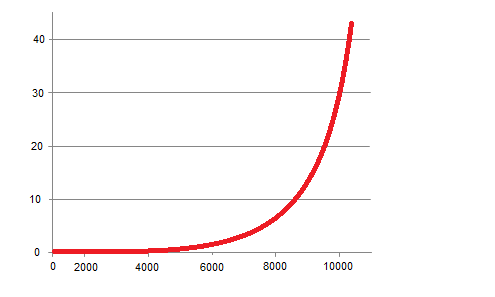
\includegraphics{Alg2Log.png}
\caption{Algorithm 2 Run Time}
\end{figure}


\subsection{Extrapolation and Interpretation}
\subsubsection{For each algorithm use the experimental data to estimate a function that models the relationship between running times and input sizes (n). Discuss any discrepancies between the experimental and theoretical running times.}

\subsubsection{For each algorithm, what is the size of the biggest instance that you can solve with your algorithm in one hour?}

\section{Algorithm 3: Divide and Conquer}

\subsection{Theoretical Run-Time Analysis}

\subsection{Proof of Correctness}

\subsection{Experimental Analysis}

\begin{figure}
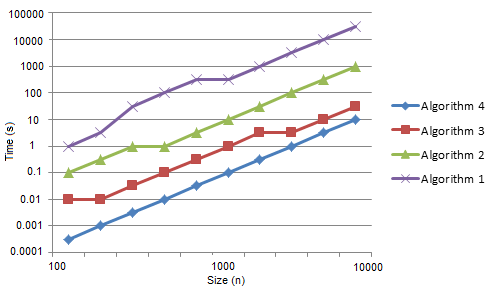
\includegraphics{AvgRunTime.png} 
\caption{Average Run Time for All 4 Algorithms}
\end{figure}
\break
\begin{figure}
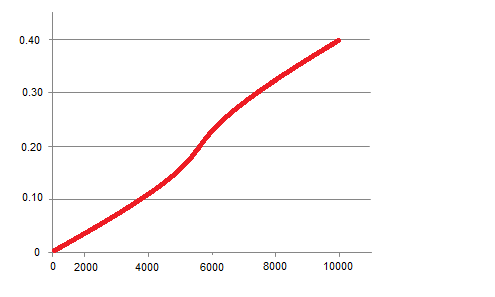
\includegraphics{Alg3Log.png}
\caption{Algorithm 3 Run Time}
\end{figure}


\subsection{Extrapolation and Interpretation}
\subsubsection{For each algorithm use the experimental data to estimate a function that models the relationship between running times and input sizes (n). Discuss any discrepancies between the experimental and theoretical running times.}

\subsubsection{For each algorithm, what is the size of the biggest instance that you can solve with your algorithm in one hour?}

\section{Algorithm 4: Linear-Time}
\subsection{Theoretical Run-Time Analysis}

\subsection{Experimental Analysis}
\begin{figure}
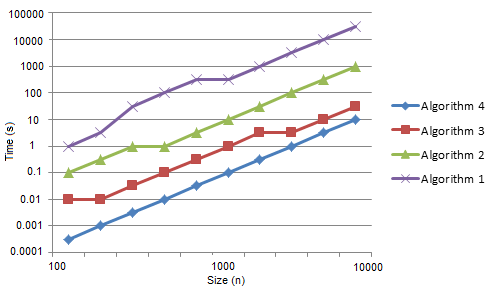
\includegraphics{AvgRunTime.png} 
\caption{Average Run Time for All 4 Algorithms}
\end{figure}
\break
\begin{figure}
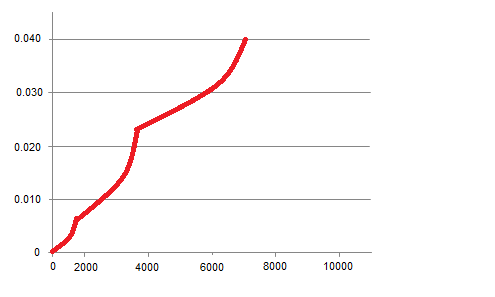
\includegraphics{Alg4Log.png}
\caption{Algorithm 4 Run Time}
\end{figure}


\subsection{Extrapolation and Interpretation}
\subsubsection{For each algorithm use the experimental data to estimate a function that models the relationship between running times and input sizes (n). Discuss any discrepancies between the experimental and theoretical running times.}

\subsubsection{For each algorithm, what is the size of the biggest instance that you can solve with your algorithm in one hour?}

\newpage{}
\section{Appendices}
\subsection{Code}
\subsubsection{Algorithm 1}
\lstinputlisting[language=Python]{algorithm1.py}
\subsubsection{Algorithm 2}
\lstinputlisting[language=Python]{algorithm2.py}
\subsubsection{Algorithm 3}
\lstinputlisting[language=Python]{algorithm3.py}
\subsubsection{Algorithm 4}
\lstinputlisting[language=Python]{algorithm4.py}

\subsection{Tests}
\lstinputlisting[language=Python]{main.py}		

\end{document}  